\documentclass[12pt]{article}

\usepackage{amsmath}
\usepackage{amssymb}
\usepackage{calc}
\usepackage{units}
\usepackage{graphicx}
\usepackage{subfig}
\usepackage[margin=1in]{geometry}
\usepackage{listings}
\usepackage[numbers,sort&compress]{natbib}
\usepackage{bm}
\usepackage{paralist}
\usepackage[draft]{fixme}

\title{Measuring Electric Phenomena:\\the Ammeter and Voltmeter}
\author{}
%Kevin R. Lynch, based on an earlier lab by Duli Jain
%\date{2012-01-24}
\date{}

\begin{document}

\maketitle

\section{Objectives}
\label{sec:objectives}

\begin{enumerate}
\item To understand the use and operation of the Ammeter and
  Voltmeter in a simple direct current circuit, and
\item To verify Ohm's Law for the resistor.
\end{enumerate}

\section{Introduction}
\label{sec:introduction}

The German physicist, Georg Ohm, was the first to explore the
relationship between the current \textit{through} an object compared
to the voltage applied \textit{across} that object.  He published his
results, \textit{Die galvanische Kette, mathematisch
  bearbeitet}\footnote{The galvanic circuit investigated
  mathematically}, in 1827.  His results were not immediately
accepted, because his methods were so revolutionary, and challenged
the accepted requirements of scientific reasoning of his day; science
is a human endeavor, and this result has a fascinating backstory that
I urge you to investigate.

To investigate the properties of voltage and current, and the
relationship between the two, we need tools and equipment to do it.
We measure voltage with the \textit{voltmeter}, and current with the
ampmeter or \textit{ammeter}.  In a later lab, you will study the
detailed properties of ideal meters, and contrast them with the real
meters that we can actually build.  In this lab, however, you will
learn the proper use of these devices while investigating Ohm's Law.

\section{Theory}
\label{sec:theory}

Ohm showed that a \textit{steady} current was caused by a
\textit{constant} voltage, and that were directly proportional to each
other, and scaled with the length of the \textit{resistive} element
through which the current flowed.  Today, we express this relationship
mathematically as $V/I \propto 1$, where $V$ is the voltage (measured
in the SI system in \textit{volts}, $V$) and $I$ is the current
(measured in \textit{amperes}, $A$).  We give the \textit{constant of
  proportionality} the name \textit{resistance}, and the symbol $R$
\begin{gather*}
  \frac{V}{I} = R\ ,
\end{gather*}
Resistance is measured in \textit{ohms}, with the symbol $\Omega$.

In this lab, the resistance $R$ will be constant for a given object.
Later, we will investigate the limits of this relationship: under what
conditions does it hold true, when does it fail, and how can we
understand these properties as the results of microscopic physics.

Let's now introduce the voltmeter and the ammeter.  A voltmeter is
designed to measure the voltage \textit{across} a portion of a
circuit, while an ammeter is designed to measure the current
\textit{passing through} a particular point in the circuit.  That is,
the voltmeter stays \textit{outside} the circuit, while the ammeter
must be inserted \textit{into} the circuit.  While these devices have
distinct properties and uses, the ammeter and voltmeter are such a
basic part of the scientific measurement toolkit, that the are usually
found integrated into a single device called the \textit{multimeter}.
There are many kinds of multimeters: desktop or handheld, analog or
digital, manual or autoranging, low and high voltage, etc.  Beware,
however!  Switching a multimeter from ammeter to voltmeter mode
usually requires the inputs to be rewired; failing to do so can result
in blown fuse, or damaging the device.  And finally, for safety
reasons, never use a multimeter for measurements in high voltage
circuits, unless you have been specifically trained for that task!  We
won't be exposing you to such risks in this course.

In order to talk in more detail about these devices, we need a
language describe the connections between them in a particular
\textit{electrical circuit} - the circuit diagram, or schematic.
Schematics are a kind of descriptive map: they make explicit the wired
connections between electrical devices in a circuit.  They are,
however, not a photograph.  The connections between devices in a
diagram do not indicate literal wires, but only topological
connections between devices.  There may be multiple physical
realizations, or \textit{layouts}, of a given schematic, and there may
be multiple equivalent schematics for a given layout.

\begin{table}
  \centering
  \begin{tabular}{|l|c|}\hline
    Resistor & 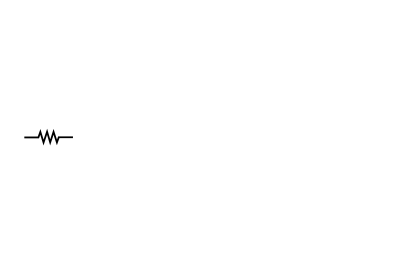
\includegraphics[width=1in]{figures/resistor}\\ \hline
    Voltmeter & 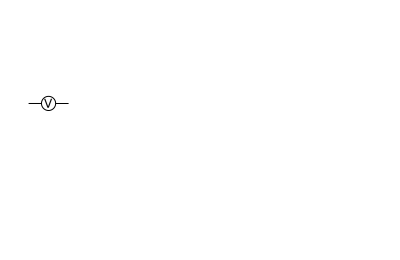
\includegraphics[width=1in]{figures/voltmeter}\\ \hline
    Ammeter & 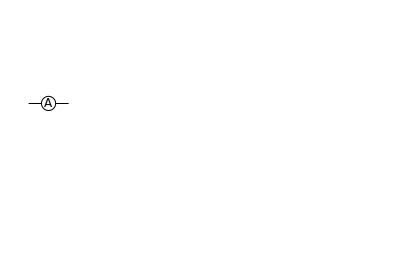
\includegraphics[width=1in]{figures/ammeter} \\ \hline
    DC Voltage source & 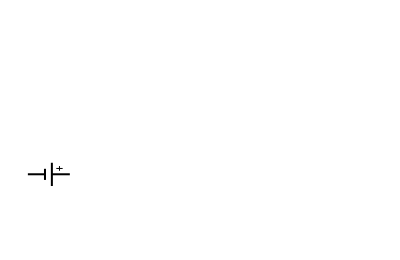
\includegraphics[width=1in]{figures/dc_supply}\\ \hline
  \end{tabular}
  \caption{The various schematic elements used in this lab.}
  \label{tab:schematic}
\end{table}
The language of circuit schematics is highly evolved, and there are de
facto standard representations of typical devices.
Table~\ref{tab:schematic} contains the common symbols used in this
lab.  

When learning to build or ``wire'' a circuit from a schematic, it is
usually best to arrange your physical devices (resistors, power
supplies, meters, etc.) in the same orientation as the devices on the
schematic.  Then, follow the ``map'' given by the schematic: pick one
terminal on the first device, and locate all the terminals on other
devices that are connected to that terminal all the schematic.  Using
one or more wires, reproduce those schematic connections in the
physical world.  Repeat until you have ``visited'' all terminals on
the schematic.  Note that not all terminals may be labeled identically
on the schematic and on the physical devices: they may be labeled
same, differently, or perhaps not labeled at all!  You will need to
use your judgment, ask questions of your instructor, or simply try
an experiment to figure things out on your own.

\section{Procedures}
\label{sec:procedures}

In this lab, we will investigate the relationship between current and
voltage in the simplest possible circuit, consisting of a direct
current voltage source and a single resistance
(Figure~\ref{fig:simple}).
\begin{figure}
  \centering
  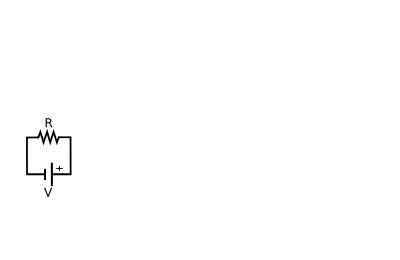
\includegraphics[width=\textwidth/5]{figures/simplest}
  \caption{The simplest direct current circuit.}
  \label{fig:simple}
\end{figure}
\begin{figure}
  \centering
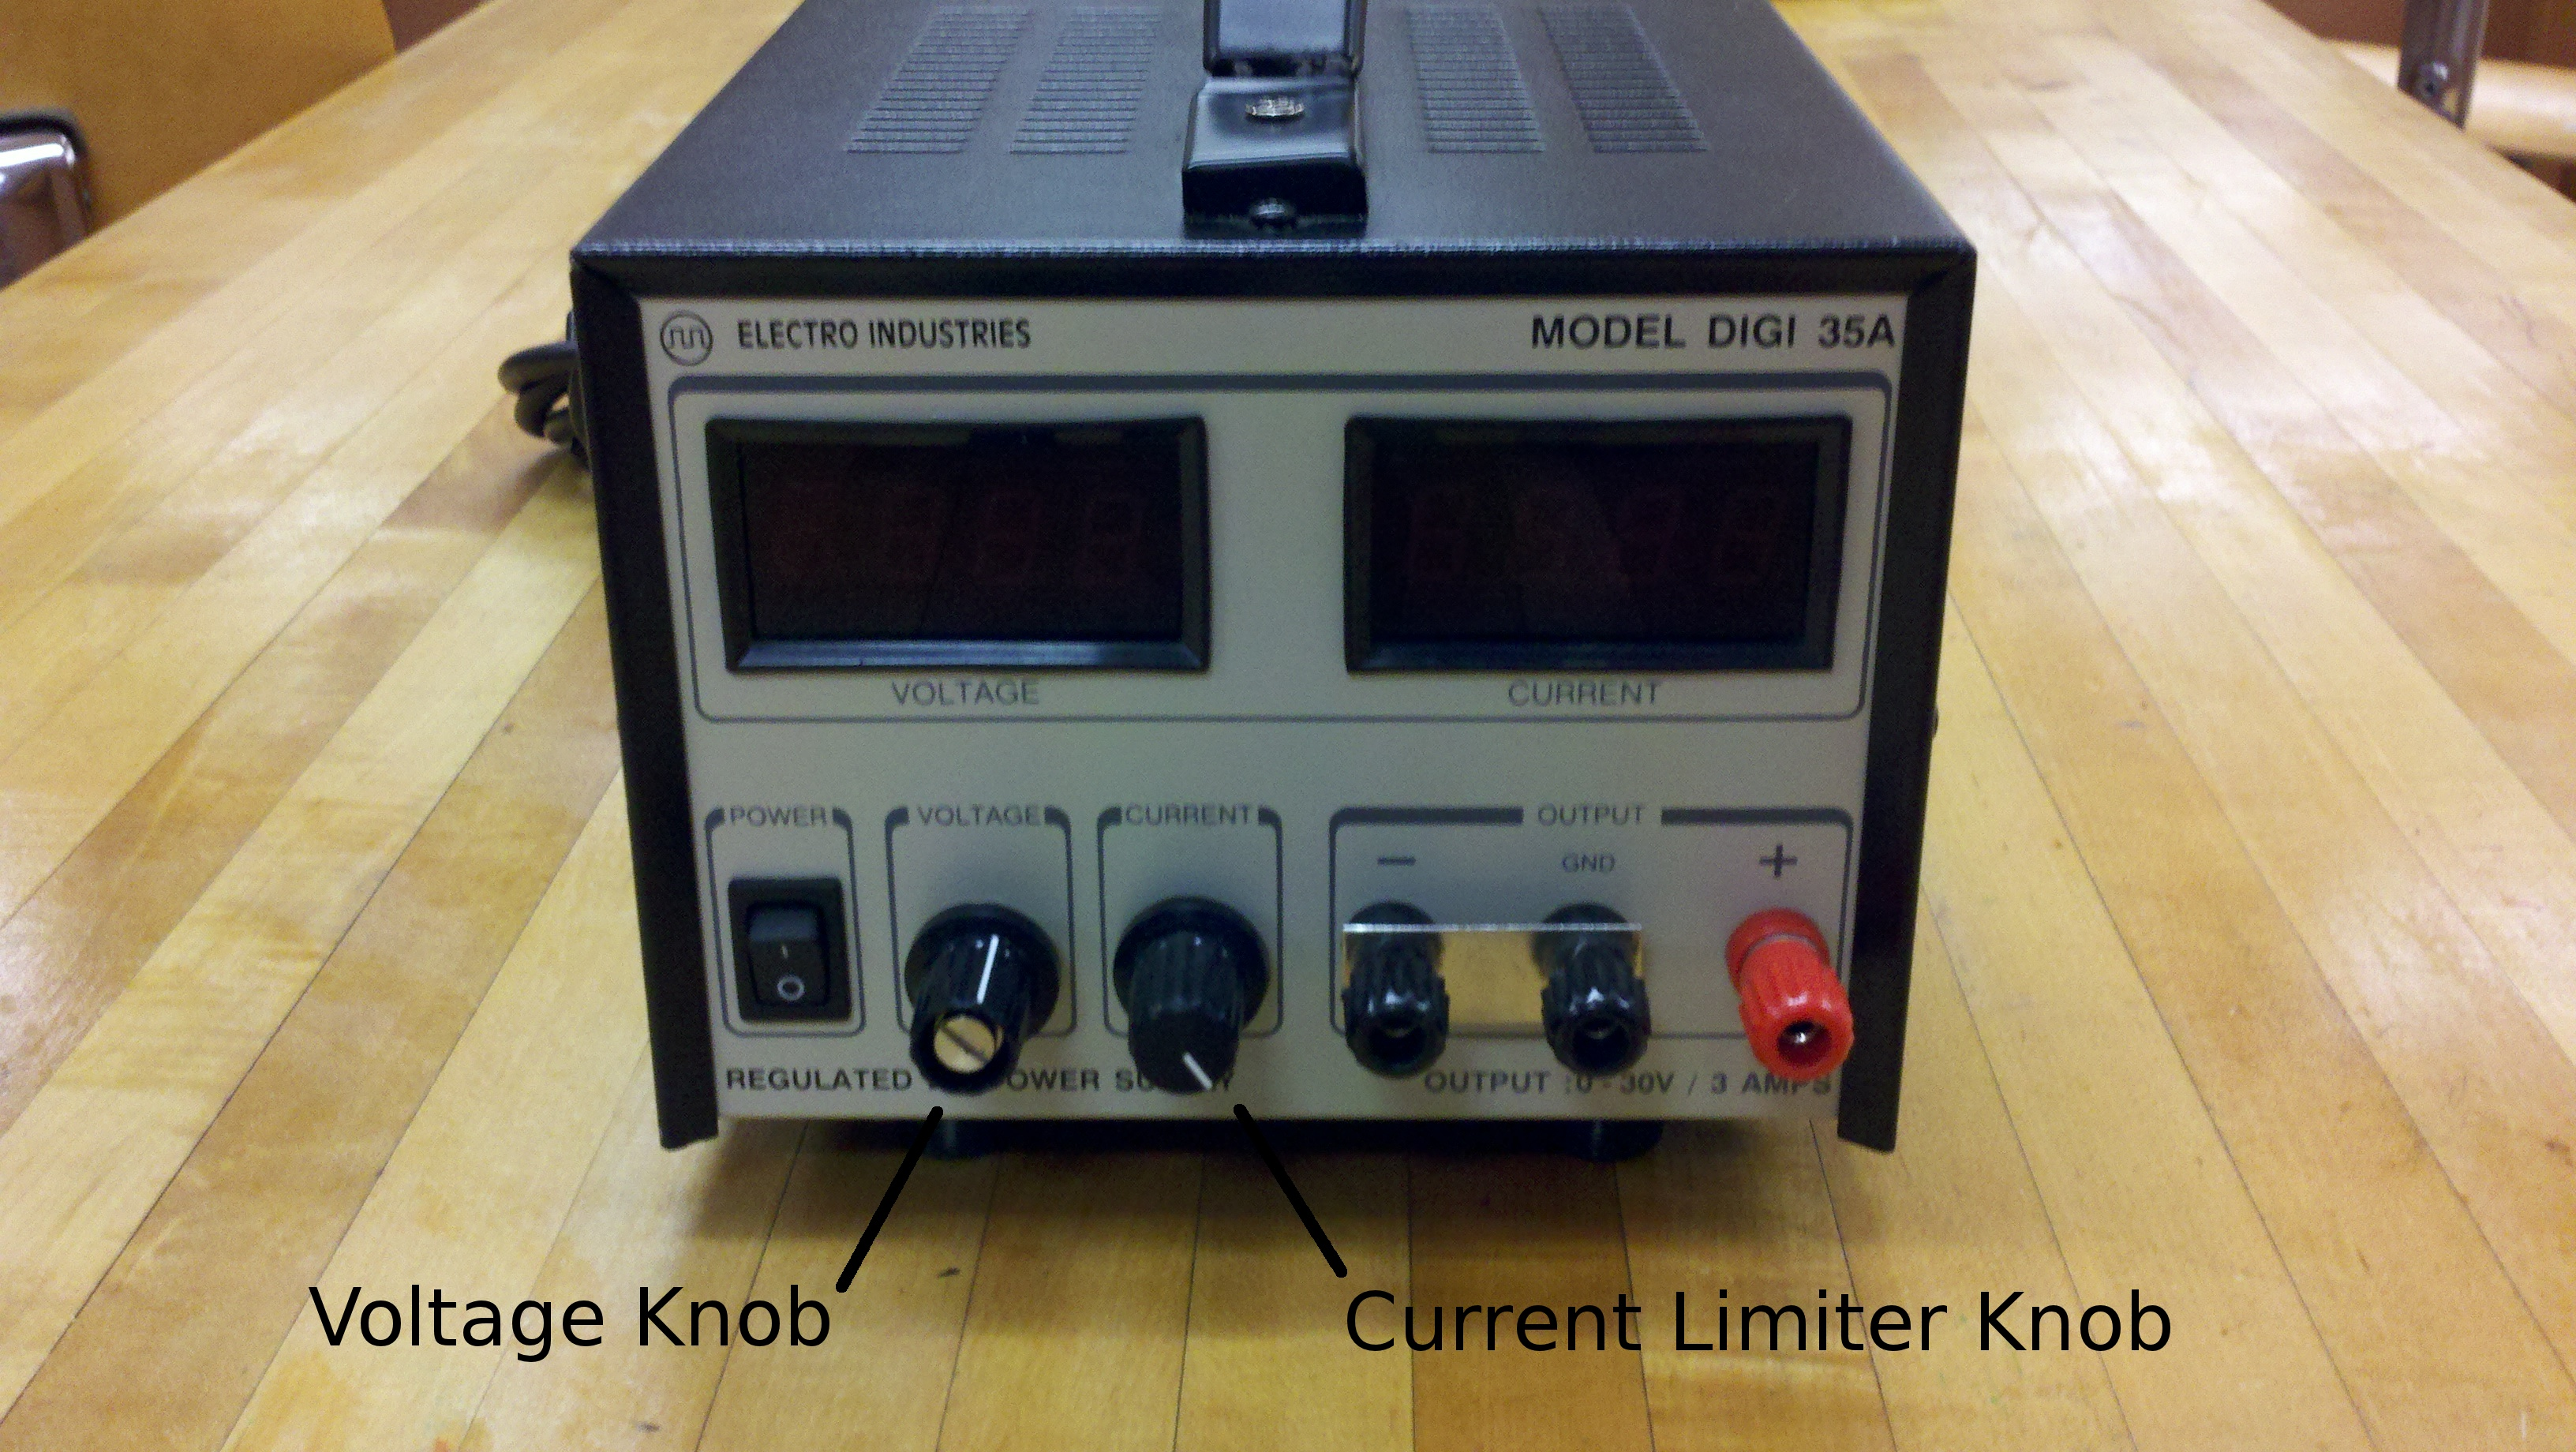
\includegraphics[width=\textwidth/2]{figures/electro_digi35a_labeled}
  \caption{The direct current power supply.}
  \label{fig:dcps}
\end{figure}
\begin{figure}
  \centering
  \subfloat[][Settings for voltmeter mode]{
    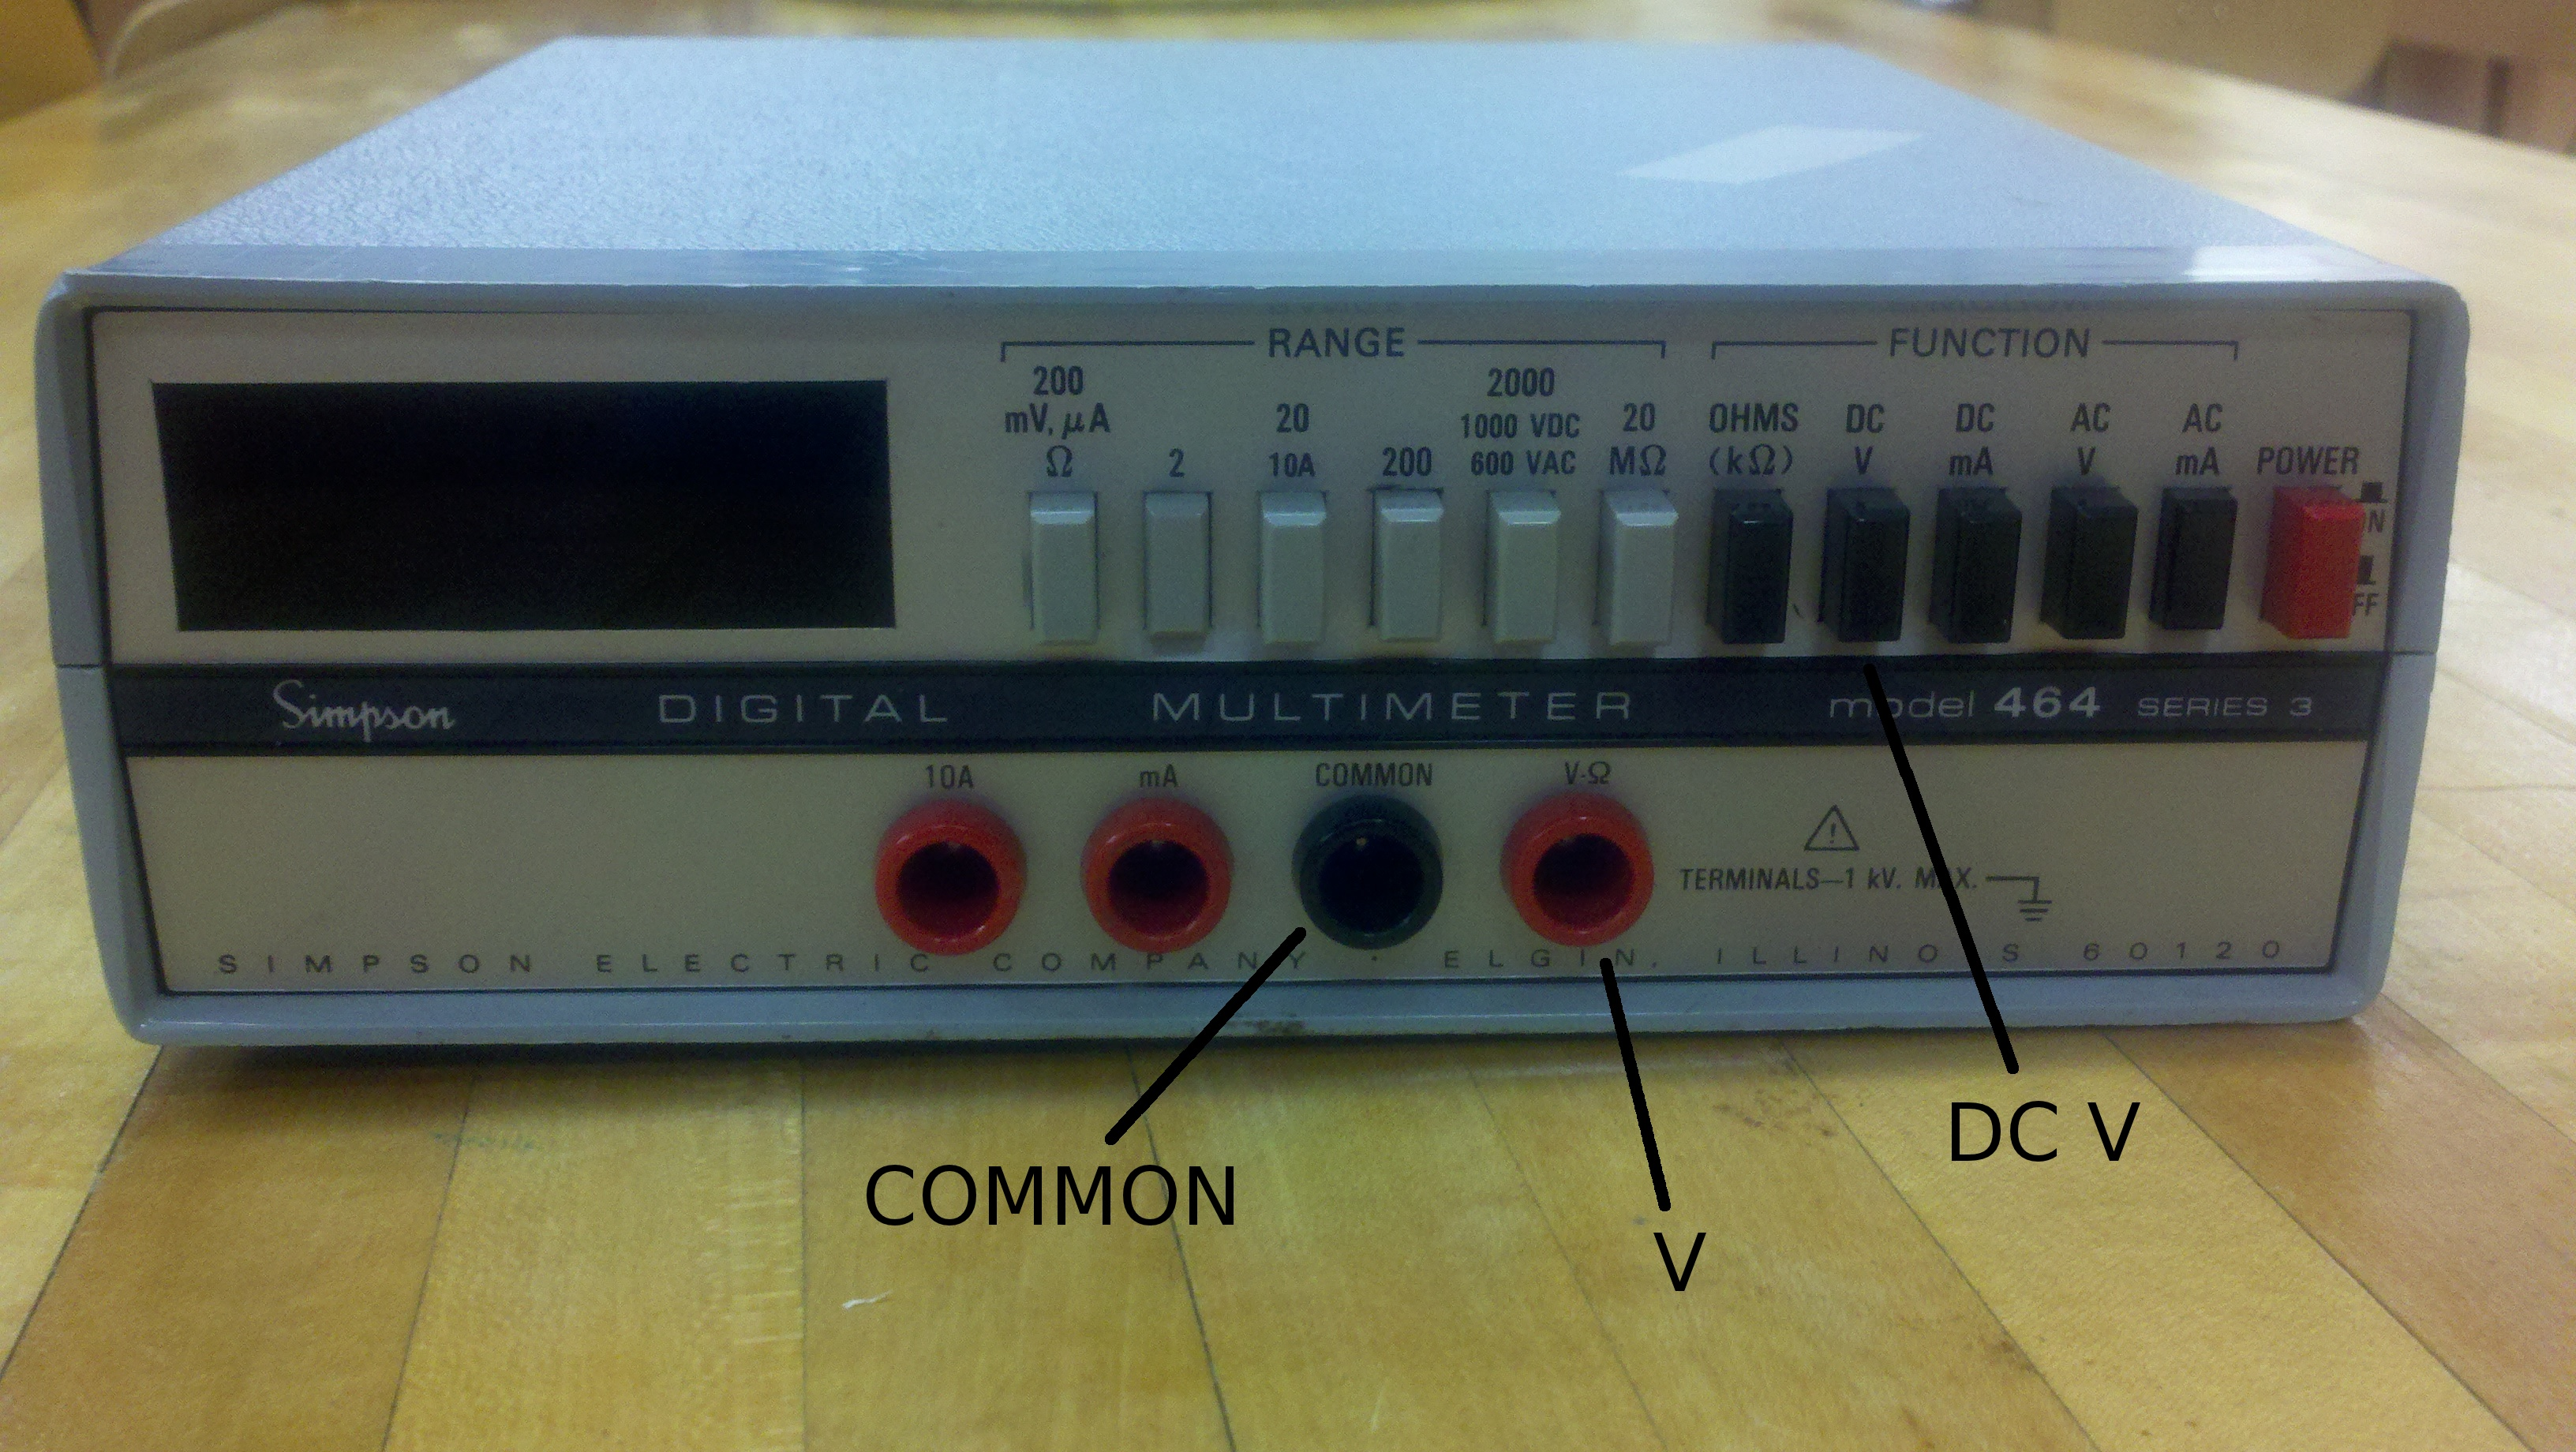
\includegraphics[width=\textwidth/3]{figures/simpson_464_voltmeter}
  }\qquad
  \subfloat[][Settings for ammeter mode]{
    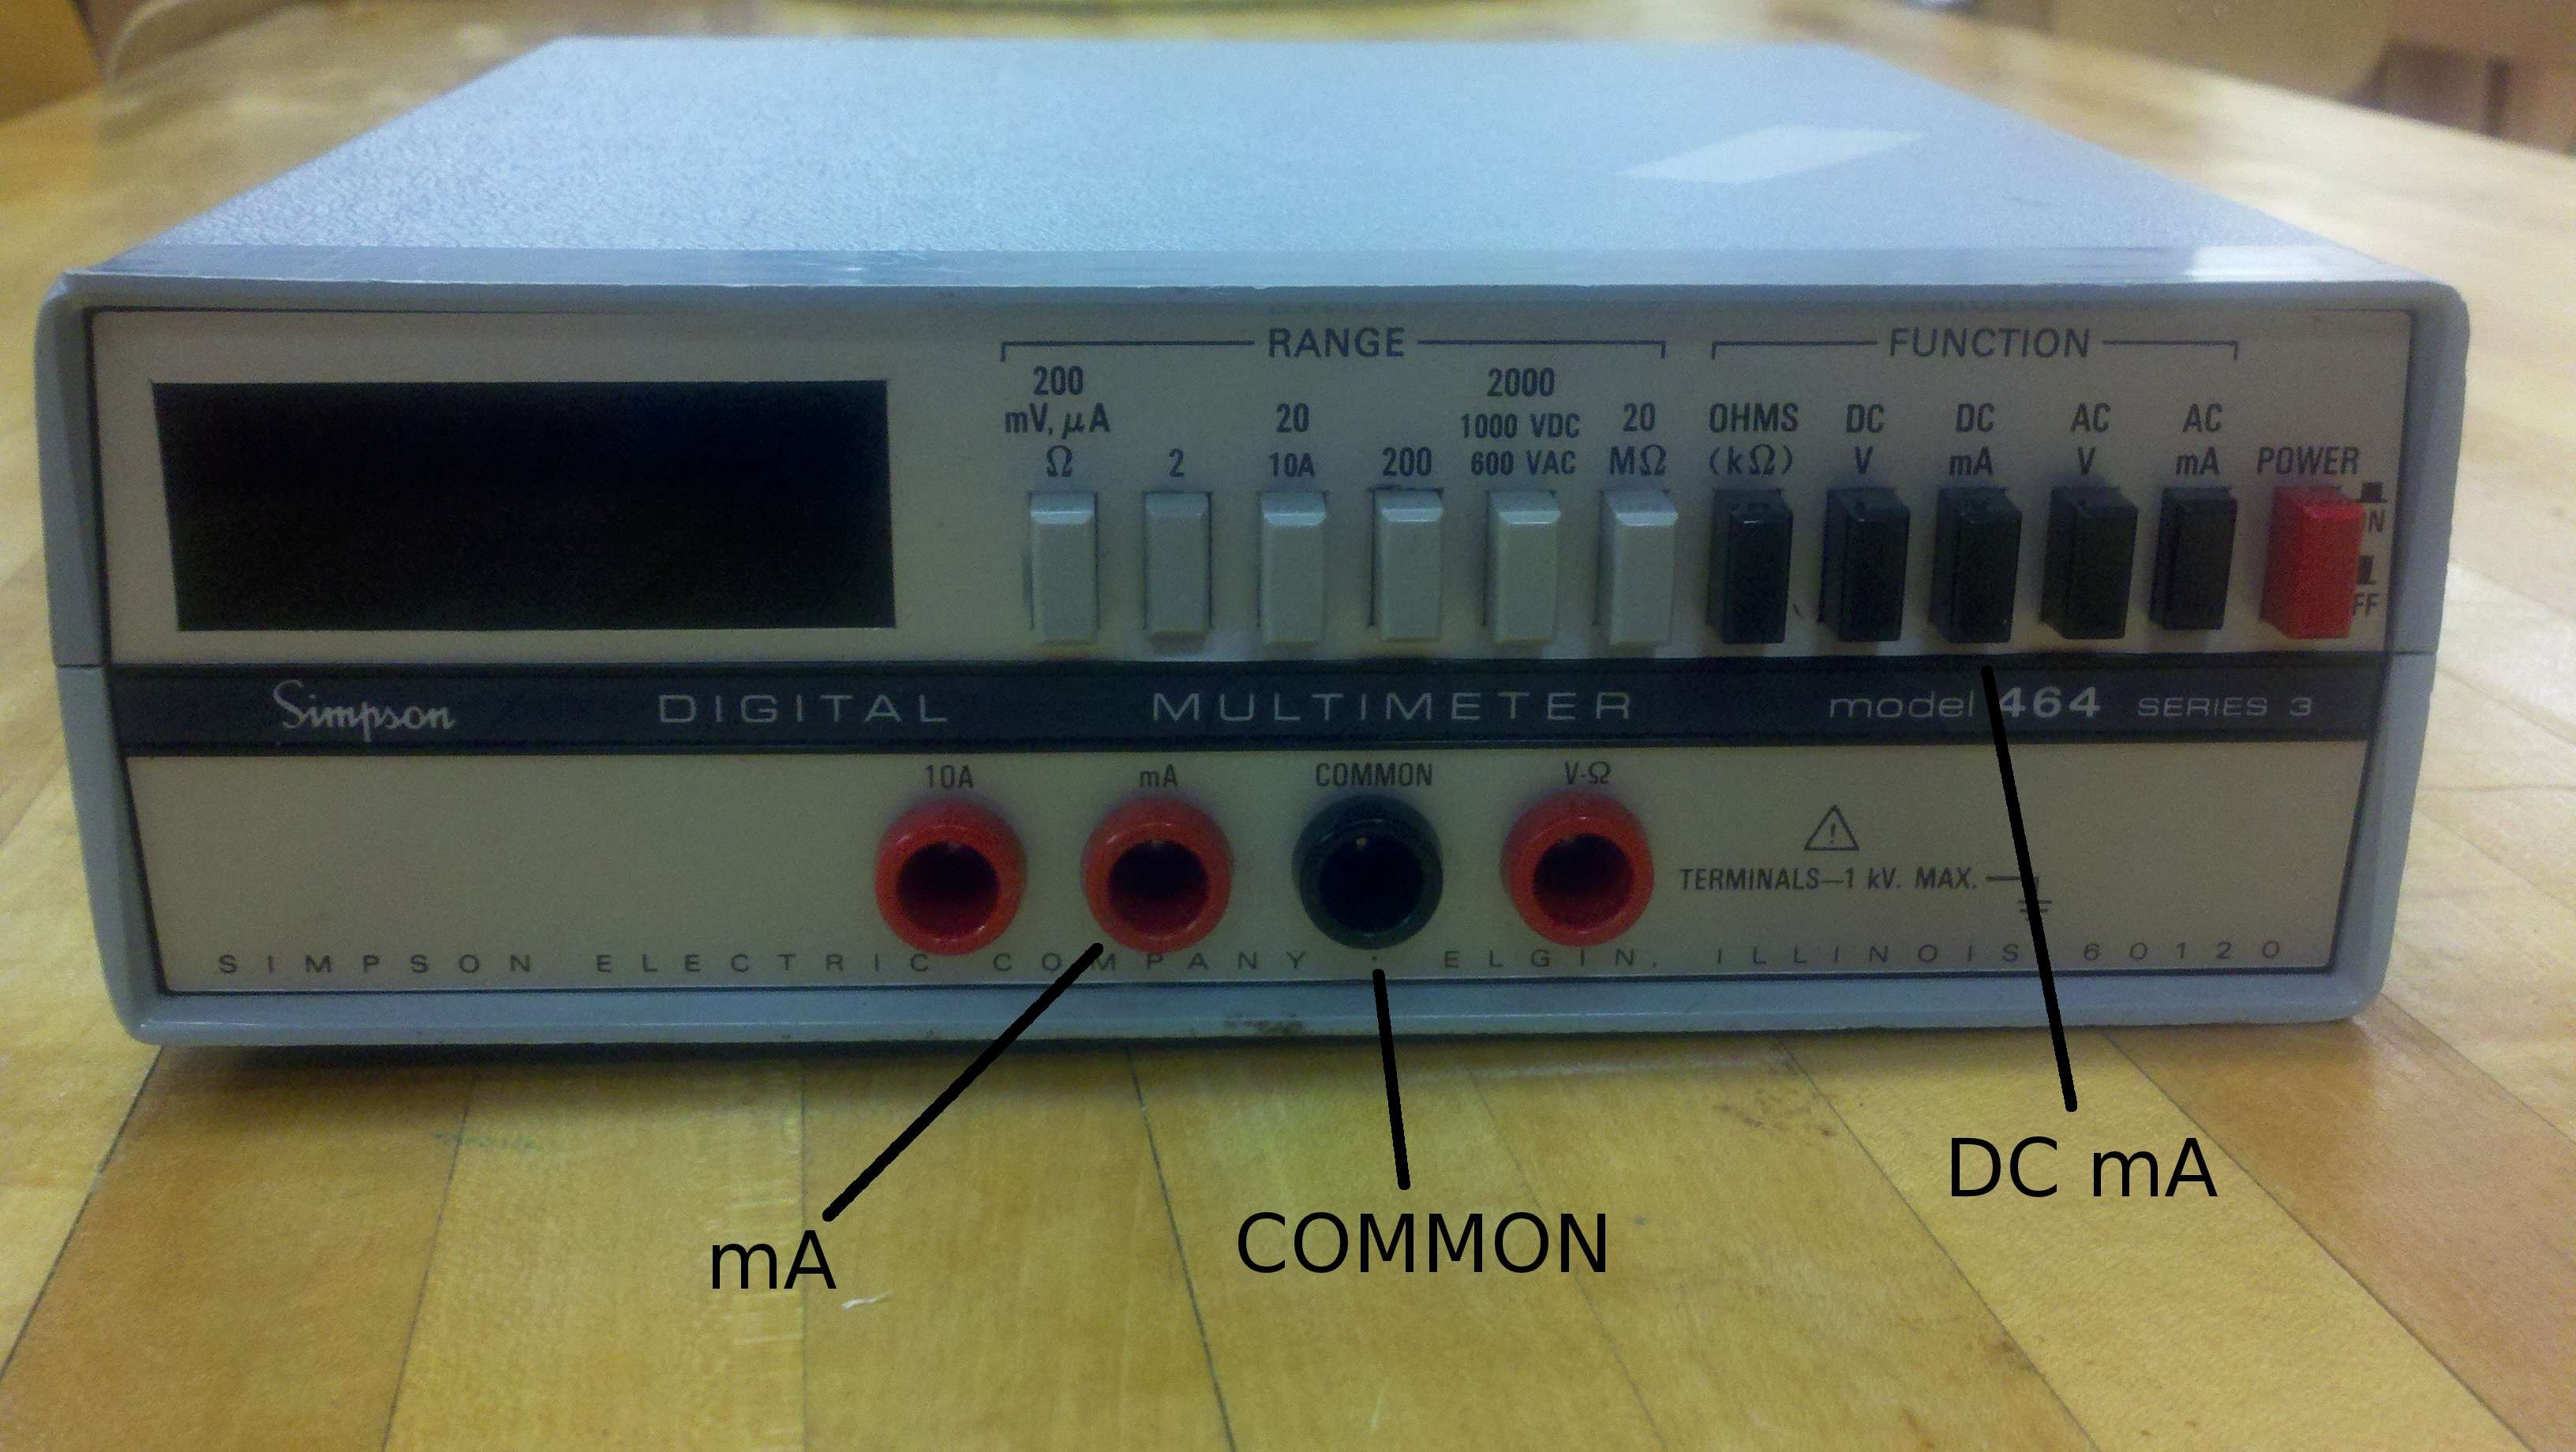
\includegraphics[width=\textwidth/3]{figures/simpson_464_ammeter}
  }  
  \caption{The multimeter.}
  \label{fig:multimeter}
\end{figure}
\begin{enumerate}
\item First, construct the circuit shown in Figure~\ref{fig:simple},
  turn the \texttt{Voltage} knob on the power supply
  (Figure~\ref{fig:dcps}) to its minimum setting (fully counter
  clockwise), and the\texttt{Current} limiter knob to its maximum
  setting (fully clockwise).  Plug in and turn on the power supply.
\item Next, configure your first multimeter as a voltmeter: connect
  your test leads to the \texttt{COMMON} and \texttt{V} inputs, and
  select the \texttt{DCV} (Direct Current Voltage) Function.  Plug in
  and turn on the multimeter.
\item 
  \begin{figure}
    \centering
    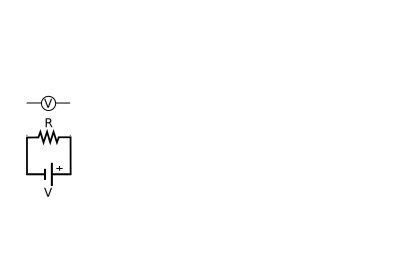
\includegraphics[width=\textwidth/5]{figures/simplest_with_voltmeter}
    \caption{The simplest direct current circuit, with voltmeter installed.}
    \label{fig:simplest_with_voltmeter}
  \end{figure}
  We'll now get a feel for how the meter works.  First, connect the
  test leads to opposite ends of the resistor - that is,
  \textit{across}) the resistor (Figure~).  To make a measurement, you
  must select the correct \texttt{RANGE}; the meter will measure
  values from \unit[0]{V} up to the value specified above the
  \texttt{RANGE} button: \unit[2]{V} for the 2 button, \unit[20]{V}
  for the 20 button, etc.  For maximum precision, always choose the
  smallest \texttt{RANGE} value larger than the voltage you are
  measuring.  When in doubt, start at the largest setting, and work
  you way down.  What happens when you go to far?

  Now, raise the voltage on the power supply; If you have connected
  the circuit and meter correctly, you should see the voltage display
  on the power supply increase from zero, and the value on the
  multimeter should roughly match that on the supply.  If not, you did
  something wrong and should ``debug'' your connections to make sure
  they are correct.  What happens when you swap the leads connected to
  the resistor?  Why?

  Turn the voltage down to zero before proceeding.
\item 
  \begin{figure}
    \centering
    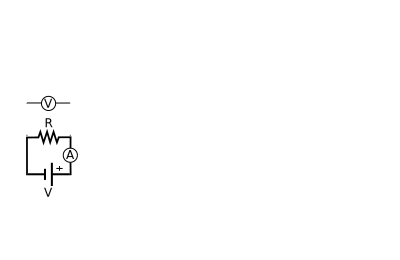
\includegraphics[width=\textwidth/5]{figures/simplest_with_ammeter}
    \caption{The direct current circuit with ammeter inserted.}
    \label{fig:simplest_with_ammeter}
  \end{figure}
  Next, configure the second multimeter as an ammeter: connect your
  test leads to the \texttt{COMMON} and \texttt{mA} inputs, and select
  the \texttt{DCmA} (Direct Current milliAmps) Function.  Again, you
  must choose an appropriate \texttt{RANGE}.  You measure current
  \textit{through} a device, which means you must insert the meter
  \textit{into} the circuit: you must ``cut'' the circuit, and
  ``splice'' the meter into the ``hole''.  In this case, you should
  insert the meter between the output of the power supply and the
  resistor.  Make sure the voltmeter is still connected across the
  resistor.  At this point, you should have recreated the circuit in
  Figure~\ref{fig:simplest_with_ammeter}.  Again, slowly raise the
  voltage output, and observe the changes in the voltage and current
  values as measured on the respective meters.
\item We are ready to repeat Ohm's measurements!  Vary the voltage in
  small steps (say, ten steps from \unit[0]{V} to \unit[10]{V}), and
  record both the voltage and the corresponding current.  Don't forget
  the units!  Repeat the measurement; are your results consistent?
  Select a different resistor, and repeat your measurements.  Plot
  your data, $I$ vs $V$: if Ohm was right, this should be linear.  Is
  it?  What is the slope?  How is this related to $R$?
\item Finally, we will use the multimeter in \texttt{Resistance} mode
  to confirm our results.  In this mode, the multimeter performs the
  same experiment we just did in large: it applies a known voltage,
  measures the demand current, and deduces the resistance from these
  two values.  Completely disconnect the circuit.  Connect test leads
  to the \texttt{COMMON} and \texttt{$\Omega$} inputs, select the
  \texttt{OHMS} Function, and an appropriate value for the
  \texttt{RANGE}.  Connect the leads to opposite sides of the
  resistor, and record the value.  Does the value you measured with
  the above procedure agree with the value the meter measures
  directly?
\end{enumerate}

Make sure you clean up your work space, and return every item to the
condition and location you originally found them in!

\newpage

\section*{Pre-Lab Questions}

On a separate sheet of letter-sized paper, please answer the following
questions in a neat and organized manner.  

\begin{enumerate}
\item What do you use a voltmeter for?
\item How about an ammeter?
\item If you double the resistance in a circuit while keeping the
  current unchanged, what happens to the voltage?  What if, instead,
  you keep the voltage unchanged?
\item Sketch the relationship between voltage and current implied by
  Ohm's Law.
\item You are told that a certain voltage will be between \unit[3]{V}
  and \unit[5]{V}, and are given a non-autoranging voltmeter.  If the
  range selectors are labeled \unit[200]{mV}, \unit[2]{V}, and
  \unit[20]{V}, which range do you select and why?
\end{enumerate}

\newpage

\section*{Post-Lab Questions}

\begin{enumerate}
\item Prepare a neatly organized tabulation of your recorded data.
  Make sure to label your data, and include units where appropriate.  
\item Plot all of your data sets on a single graph, preferably by
  computer.  Does your data support or refute Ohm's Law?  Why or why
  not?  How do you determine the value of the resistance from your
  plot?  Does it agree with the values you measured directly with the
  multimeter?  Why or why not?
\item Imagine you have a circuit consisting or two resistors and one
  power supply.  How many different ways are there to connect these
  elements into a circuit?  Draw schematics for all the possible
  inequivalent circuits.  Make sure to label the components.  For one
  of these circuits, draw a new diagram showing how you would connect
  a multimeter to measure the voltage across the power supply, and
  another to show how you would measure the voltage across one of the
  resistors.
\item Discuss briefly whether you have met the objectives of the lab
  exercises.  
\end{enumerate}

\end{document}

%%% Local Variables: 
%%% mode: latex
%%% TeX-master: t
%%% End: 
